

%%%%%%%%%%%%%%%%%%%%%%%%%%%%%%%

\begin{frame}{The Big Picture}
  \frame{\includegraphics[angle=270,width=1.0\textwidth]{figures/openmp-big-picture}} \\
  {\scriptsize ``OpenMP Basics and MPI/OpenMP Scaling'', Yun He, NERSC, 2015}  
\end{frame}

\begin{frame}{The Big Picture}
  \frame{\includegraphics[angle=270,width=1.0\textwidth]{figures/nwchem-mpi-openmp}} \\
  {\scriptsize ``OpenMP Basics and MPI/OpenMP Scaling'', Yun He, NERSC, 2015}  
\end{frame}

\begin{frame}{The Big Picture}
  \frame{\includegraphics[angle=270,width=1.0\textwidth]{figures/openmp-fun}} \\
  {\scriptsize ``OpenMP Basics and MPI/OpenMP Scaling'', Yun He, NERSC, 2015}  
\end{frame}

\begin{frame}{Future Systems}
  \includegraphics[width=1.0\textwidth]{figures/ASCR-Upgrades.png}
\end{frame}


\begin{frame}{Future Systems}

\begin{minipage}{0.6\textwidth}
 \begin{block}{Some Systems are Hybrid}
  \begin{itemize}
   \item Multi-core CPUs + many-core GPUs
   \item Multi-core CPUs + FPGAs?
   \item Multi-core CPUs + custom accelerators?
  \end{itemize}
 \end{block}

  \begin{block}{Why MPI+X for Hybrid Systems?}
  \begin{itemize}
   \item MPI not available on GPUs/FPGAs/accelerators
  \end{itemize}
 \end{block}
\end{minipage}
\begin{minipage}{0.39\textwidth}
 \includegraphics[width=1.0\textwidth]{figures/mpi_cuda} \\
 {\scriptsize \hspace*{-3.5cm} \texttt{http://geco.mines.edu/tesla/cuda\_tutorial\_mio/pic/mpi\_cuda.jpg} }
\end{minipage}

\begin{center}
 \includegraphics[height=1.1cm]{figures/cuda-logo} \
 \includegraphics[height=1cm]{figures/openmp_logo} \
 \includegraphics[height=1.5cm]{figures/opencl}
\end{center}


\end{frame}


%%%%%%%%%%%%%%%%%%%%%%%%%%%%%%%

\begin{frame}{Simple MPI Model}
\begin{center}
  \includegraphics[width=0.8\textwidth]{figures/simple-mpi}
\end{center}
\begin{block}{Hybridization Easy?}
 \begin{itemize}
   \item \texttt{\#pragma omp parallel for}
 \end{itemize}
\end{block}
\end{frame}



\begin{frame}{Simple MPI Model}
 \begin{minipage}{0.55\textwidth}
  \begin{block}{Mind the Details}
   \begin{itemize}
    \item NUMA domains: Data locality matters
    \item CPU internals: Ring buses
   \end{itemize}
  \end{block}
 \end{minipage}

  \begin{center}
   \includegraphics[width=0.75\textwidth]{figures/BroadwellXeonSchematic} \\
   {\scriptsize \texttt{http://images.anandtech.com/doci/10158/v4\_24coresHCC.png} }
  \end{center}

\end{frame}


%%%%%%%%%%%%%%%%%%%%%%%%%%%%%%%

\begin{frame}{NUMA-aware MPI Model}
  \includegraphics[width=1.0\textwidth]{figures/numa-mpi}
\end{frame}

\begin{frame}{Hybrid MPI Model}
  \begin{block}{Hybridization}
   \begin{itemize}
    \item One or multiple multi-core CPUs
    \item One or multiple GPUs/FPGAs/accelerators
   \end{itemize}
  \end{block}

  \begin{block}{CPU Starvation}
   \begin{itemize}
    \item Use one MPI rank per GPU (shepard process)
    \item Problem: Waste of CPU resources
   \end{itemize}
  \end{block}

\end{frame}

%%%%%%%%%%%%%%%%%%%%%%%%%%%%%%%

\begin{frame}{GPUs in the MPI Model}
  \includegraphics[width=1.0\textwidth]{figures/gpu-mpi}
\end{frame}


\begin{frame}{GPUs in the MPI Model}
  \includegraphics[width=1.0\textwidth]{figures/hybrid-mpi}
\end{frame}

%%%%%%%%%%%%%%%%%%%%%%%%%%%%%%%


\begin{frame}[fragile]{Reflection}

 \begin{block}{MPI+X for Hybrid Systems}
  \begin{itemize}
   \item Important question: What to compute where?
   %\pause
   \item Unimportant question: What is X?
  \end{itemize}
 \end{block}
 
 %\pause
 
 \begin{center}
  \includegraphics[width=0.99\textwidth]{figures/spgemm-crop}
 \end{center}

\end{frame}



%% Memory bandwidth vs. Parallelism


\begin{frame}{PCI-Express Bottleneck}

 \begin{block}{Vector Addition}
  \begin{itemize}
   \item $x = y + z$ with $N$ elements each
   \item 1 FLOP per 24 byte in double precision
   \item Limited by memory bandwidth $\Rightarrow T_2(N) \stackrel{?}{\approx} 3 \times 8 \times N / \mathrm{Bandwidth} + \mathrm{Latency}$
  \end{itemize}
 \end{block}

 \vspace*{-0.5cm}
 \begin{center}
  \includegraphics[width=0.75\textwidth]{figures/vector-addition-time-3}
 \end{center}
 
 \end{frame}



\begin{frame}{PCI-Express Bottleneck}
  \includegraphics[width=1.0\textwidth]{figures/time-laplace2d-K20m-cg}
\end{frame}

\begin{frame}{PCI-Express Bottleneck}
  \includegraphics[width=1.0\textwidth]{figures/amg-vs-pure-full-2d}
\end{frame}


\begin{frame}{PCI-Express Bottleneck}
  \begin{minipage}{0.55\textwidth}
    \begin{block}{Example: Algebraic Multigrid}
     \begin{itemize}
      \item SpGEMM on CPU (AMG setup)
      \item SpMV \& friends on GPUs (AMG solve)
     \end{itemize}
    \end{block}
    
    %\visible<2->{
     \begin{block}{Model 1: Side-by-Side}
     \begin{itemize}
      \item Use MPI ranks for CPU
      \item How to decompose problem?
     \end{itemize}
    \end{block}%}

    %\visible<3->{
    \begin{block}{Model 2: GPU shepards only}
     \begin{itemize}
      \item Overlapping of GPU and CPU work within rank
      \item Reimplement message passing on MPI rank level?
     \end{itemize}
    \end{block}
    %}
  \end{minipage}
  \begin{minipage}{0.44\textwidth}
  \includegraphics[width=1.0\textwidth]{figures/amg-cpu-gpu.png} \\
  {\scriptsize N.~Bell \textit{et al.}, SISC 34(4), 2012}
  \end{minipage}
\end{frame}
